\section{Intermezzo}
\label{sec:intermezzo}

\begin{frame}
	\frametitle{Intermezzo: Strings}
	\framesubtitle{Spoiler warning: they are terrible}

	\begin{columns}
		\column{0.455\textwidth}
			\lstinputlisting{code/string_terrible.py}
		\column{0.455\textwidth}
			\begin{alertblock}{Pretty bad}
				For every append, we claim a new array. So this is $O(n^2)$ time!
			\end{alertblock}	
	\end{columns}
\end{frame}

\begin{frame}
	\frametitle{How do we solve that?}
	\begin{questionblock}{Can we do better?}
		Can we not just do this in linear time? Can we not do better?
	\end{questionblock}
	\pause
	\begin{answerblock}{Well...}
		Yes we can do it in linear time? Is that better, well yes in terms of time spent\dots\\
		No in terms of readability.
	\end{answerblock}
\end{frame}

\begin{frame}
	\frametitle{Linear time string copy}
	
	\begin{columns}
		\column{0.455\textwidth}
			\lstinputlisting{code/string_linear.py}
		\column{0.455\textwidth}
				\begin{exampleblock}{Exploiting amortisation}
					We now use the amortised effects of the list.
				\end{exampleblock}			
	\end{columns}
\end{frame}

\begin{frame}
	\frametitle{Getting rid of the intermediate list in Python}
		\begin{exampleblock}{Generator comprehension}
			Might as well take this to it's final form.
		\end{exampleblock}	
		\lstinputlisting{code/string_linear_gen.py}
		\pause
			\begin{alertblock}{In C\dots}
				Actually in the underlying C code that is used, nothing has changed :(
			\end{alertblock}	
\end{frame}

\begin{frame}
	\frametitle{Long story short}
	\framesubtitle{XKCD: Python \url{https://xkcd.com/353}}
	\begin{columns}
		\column{0.455\textwidth}
	\begin{center}
		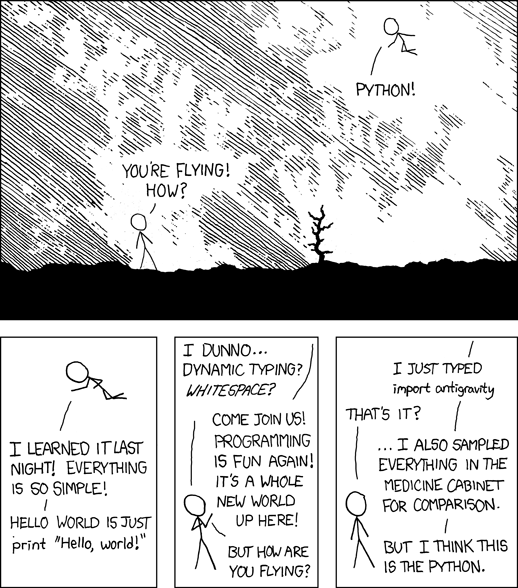
\includegraphics[width=0.9\textwidth]{figures/python.png}\\
	\end{center}
		\column{0.455\textwidth}
		\begin{itemize}
			\item Python is amazing!
				\pause
			\item Until it is not.
		\end{itemize}
	\end{columns}
\end{frame}


